\newpage
\begin{appendices}
	
\setcounter{page}{1}										% Restart page numbering
\setcounter{footnote}{0}									% Restart footnote counter
\renewcommand{\thetable}{\thesection.\arabic{table}}		% Table name aligned to appendix
\renewcommand{\thefigure}{\thesection.\arabic{figure}}		% Figure name aligned to appendix
\renewcommand{\theequation}{\thesection.\arabic{equation}}	% Equation name aligned to appendix
%	\captionsetup[table]{name=Table A}						% Change table caption prefix

\section{Section} % \label{sec:appdx1}
\vspace{0.7cm}
\iftoggle{toclinks}{\gototoc}{} 							% Turn it on/off in packages.tex
\iftoggle{cboxes}{	   				  						% Turn it on/off in packages.tex
	\begin{boxeditems}
		\item To-do list.
	\end{boxeditems}}{}
\setcounter{table}{0}
\setcounter{figure}{0}
\setcounter{equation}{0}

Appendix content.\footnote{Counters for pages, footnotes, figures, tables and equations are restarted.}

\begin{equation} \label{eq:ExEqN}
	\eqYP
\end{equation}
%\begin{equation*}	% Needs no label
	\eqYP
\end{equation*} use it in slides


\section{Section} % \label{sec:appdx2}
\vspace{0.7cm}
\iftoggle{toclinks}{\gototoc}{} 							% Turn it on/off in packages.tex
\iftoggle{cboxes}{	   				  						% Turn it on/off in packages.tex
	\begin{boxeditems}
		\item To-do list.
	\end{boxeditems}}{}
\setcounter{table}{0}
\setcounter{figure}{0}
\setcounter{equation}{0}

Appendix content.

\begin{multline} \label{eq:ExLongN}
	\eqLong
\end{multline}

\documentclass[a4paper,12pt]{article}
\usepackage[labelsep=period,labelfont=bf]{caption}
\usepackage[margin=1in]{geometry}
\usepackage{tabularx}
\usepackage{booktabs}
\usepackage{multirow}
\usepackage{bigstrut}
\usepackage{siunitx}
\usepackage{threeparttable}
\usepackage{afterpage}
\usepackage{pdflscape}
%% Customized Macros
% Table of Contents, Tasks, Tables, Subcaptions, Track Changes
%
%\gototoc
%\maketoc
%\begin{boxeditems} \end{boxeditems}
%\estauto
%\specialcell
%\fignotes
%\tabnotes
%\textchange

%---------------------------------------------------------------
% Table of Contents
%---------------------------------------------------------------

% Link to ToC from section
\newcommand{\gototoc}{\vspace{-2cm} \null\hfill [\hyperlink{toc}{Go2ToC}] \newline}

% Link back to section from ToC
\newcommand{\maketoc}{
	\clearpage
	\hypertarget{toc}{}
	\tableofcontents
	\thispagestyle{empty}
	\vspace{2.5\bigskipamount}
}

%---------------------------------------------------------------
% Tasks
%---------------------------------------------------------------

% Box with bullets for tasks to do in a section
\newenvironment{boxeditems}
	{\begin{tabular}{|p{\linewidth}|}
	\hline
	\begin{singlespace}
	\vspace{-0.4cm}
	\begin{itemize}
	}
	{
	\vspace{-0.4cm}
	\end{itemize}
	\end{singlespace}
	\\ \hline
	\end{tabular} \\
	}

%---------------------------------------------------------------
% Tables
%---------------------------------------------------------------

% Estout commands following Jörg Weber (https://www.jwe.cc/2012/03/stata-latex-tables-estout/)
\newcommand{\sym}[1]{\rlap{#1}}

\let\estinput=\input	% define new input command to flatten the document

\newcommand{\estauto}[2]{
	\newcolumntype{C}{>{\centering\arraybackslash}X}
	\vspace{.75ex}{
		\begin{tabularx}{0.95\linewidth}{l*{#2}C}
			\toprule
			\estinput{#1}
			\\ \bottomrule
			\addlinespace[.75ex]
		\end{tabularx}
	}
}

% Allow line breaks with \\ in table columns, e.g. mtitle("\specialcell{Co-Holding\\> \var1}")
\newcommand{\specialcell}[2][c]{\begin{tabular}[#1]{@{}c@{}}#2\end{tabular}}

%---------------------------------------------------------------
% Subcaptions
%---------------------------------------------------------------

% Notes after figures following Jörg Weber (https://www.jwe.cc/2012/03/stata-latex-tables-estout/)
\newcommand{\figtext}[1]{
	\vspace{-1ex}
	\captionsetup{justification=justified,font=footnotesize}
	\caption*{#1}
%	\captionsetup{justification=raggedright,singlelinecheck=false,font=footnotesize}
%	\caption*{\hspace{6pt}\hangindent=1.5em #1}
}

\newcommand{\fignote}[1]{\figtext{\emph{Note:~}~#1}}
\newcommand{\fignotes}[1]{\figtext{\emph{Notes:~}~#1}}

% Notes after tables
\newcommand{\tabnotes}[1]{
	\begin{tablenotes}[para,flushleft]
		\footnotesize \emph{Notes:~}~#1
	\end{tablenotes}
}

%---------------------------------------------------------------
% Track Changes
%---------------------------------------------------------------

% % Highlight changes in revised version with color
\newcommand{\textchange}[1]{\iftoggle{revised}{\textcolor{blue}{#1}}{#1}}			   			% Customized commands
%% Variable Definitions

%---------------------------------------------------------------
% General
%---------------------------------------------------------------
\providecommand{\tnr}{n}
\providecommand{\tidx}{t}
\providecommand{\Yield}{y_{\tidx, \tnr}}
\providecommand{\PriceLag}{P_{\tidx+1,\tnr-1}}

%---------------------------------------------------------------
% Math fonts
%---------------------------------------------------------------
\providecommand{\Expec}{\mathrm{E}_{\tidx}}
\providecommand{\Qmeasure}{\mathbb{Q}}

%---------------------------------------------------------------
% Greeks
%---------------------------------------------------------------
\providecommand{\error}{\nu_{\tidx}}

%---------------------------------------------------------------
% Notes
%---------------------------------------------------------------
%\providecommand defines a new command; if it is already defined, the (re)definition is ignored instead of sending an error.
			    	% Variable definitions
%\pagestyle{empty}

\begin{document}
%	\afterpage{
	\begin{footnotesize}
%		\begin{landscape}
		\begin{table}[tbph]
			\centering
			\caption{Caption} \label{tab:test}
			\begin{threeparttable}
				\begin{tabular}{lccc}
					\toprule
					& Freq. & \(H_{0}: k = k_{0}\) & Statistic \\
					\midrule
					\multirow{6}[5]{*}{Var. 1} & \multirow{3}{*}{I} & 0 & 40.12 \\
					& & 1 & 11.57 \\
					& & 2 &  0.03 \\
					\cmidrule(lr){2-4}
					& \multirow{3}{*}{D} & 0 & 41.76 \\
					& & 1 & 13.88 \\
					& & 2 &  0.07 \\
					\cmidrule(lr){1-4}
					\multirow{4}[5]{*}{Var. 2} & \multirow{2}{*}{I} & 0 & 26.47 \\
					& & 1 &  7.47 \\
					\cmidrule(lr){2-4}
					& \multirow{2}{*}{D} & 0 & 28.56 \\
					& & 1 &  9.15 \\
					\bottomrule
				\end{tabular}
				\tabnotes{Add standalone description. You can reference sections like \ref{sec:data} and variables like \lastobs.}
			\end{threeparttable}
		\end{table}
%	\end{landscape}
	\end{footnotesize}
%	}
\end{document}


\documentclass{article}
\usepackage[labelsep=period,labelfont=bf]{caption}
\usepackage[margin=1in]{geometry}
\usepackage[outdir=./]{epstopdf}
\usepackage{graphicx}
\usepackage{afterpage}
\usepackage{subcaption}
%% Customized Macros
% Table of Contents, Tasks, Tables, Subcaptions, Track Changes
%
%\gototoc
%\maketoc
%\begin{boxeditems} \end{boxeditems}
%\estauto
%\specialcell
%\fignotes
%\tabnotes
%\textchange

%---------------------------------------------------------------
% Table of Contents
%---------------------------------------------------------------

% Link to ToC from section
\newcommand{\gototoc}{\vspace{-2cm} \null\hfill [\hyperlink{toc}{Go2ToC}] \newline}

% Link back to section from ToC
\newcommand{\maketoc}{
	\clearpage
	\hypertarget{toc}{}
	\tableofcontents
	\thispagestyle{empty}
	\vspace{2.5\bigskipamount}
}

%---------------------------------------------------------------
% Tasks
%---------------------------------------------------------------

% Box with bullets for tasks to do in a section
\newenvironment{boxeditems}
	{\begin{tabular}{|p{\linewidth}|}
	\hline
	\begin{singlespace}
	\vspace{-0.4cm}
	\begin{itemize}
	}
	{
	\vspace{-0.4cm}
	\end{itemize}
	\end{singlespace}
	\\ \hline
	\end{tabular} \\
	}

%---------------------------------------------------------------
% Tables
%---------------------------------------------------------------

% Estout commands following Jörg Weber (https://www.jwe.cc/2012/03/stata-latex-tables-estout/)
\newcommand{\sym}[1]{\rlap{#1}}

\let\estinput=\input	% define new input command to flatten the document

\newcommand{\estauto}[2]{
	\newcolumntype{C}{>{\centering\arraybackslash}X}
	\vspace{.75ex}{
		\begin{tabularx}{0.95\linewidth}{l*{#2}C}
			\toprule
			\estinput{#1}
			\\ \bottomrule
			\addlinespace[.75ex]
		\end{tabularx}
	}
}

% Allow line breaks with \\ in table columns, e.g. mtitle("\specialcell{Co-Holding\\> \var1}")
\newcommand{\specialcell}[2][c]{\begin{tabular}[#1]{@{}c@{}}#2\end{tabular}}

%---------------------------------------------------------------
% Subcaptions
%---------------------------------------------------------------

% Notes after figures following Jörg Weber (https://www.jwe.cc/2012/03/stata-latex-tables-estout/)
\newcommand{\figtext}[1]{
	\vspace{-1ex}
	\captionsetup{justification=justified,font=footnotesize}
	\caption*{#1}
%	\captionsetup{justification=raggedright,singlelinecheck=false,font=footnotesize}
%	\caption*{\hspace{6pt}\hangindent=1.5em #1}
}

\newcommand{\fignote}[1]{\figtext{\emph{Note:~}~#1}}
\newcommand{\fignotes}[1]{\figtext{\emph{Notes:~}~#1}}

% Notes after tables
\newcommand{\tabnotes}[1]{
	\begin{tablenotes}[para,flushleft]
		\footnotesize \emph{Notes:~}~#1
	\end{tablenotes}
}

%---------------------------------------------------------------
% Track Changes
%---------------------------------------------------------------

% % Highlight changes in revised version with color
\newcommand{\textchange}[1]{\iftoggle{revised}{\textcolor{blue}{#1}}{#1}}			   				% Customized commands
%% Variable Definitions

%---------------------------------------------------------------
% General
%---------------------------------------------------------------
\providecommand{\tnr}{n}
\providecommand{\tidx}{t}
\providecommand{\Yield}{y_{\tidx, \tnr}}
\providecommand{\PriceLag}{P_{\tidx+1,\tnr-1}}

%---------------------------------------------------------------
% Math fonts
%---------------------------------------------------------------
\providecommand{\Expec}{\mathrm{E}_{\tidx}}
\providecommand{\Qmeasure}{\mathbb{Q}}

%---------------------------------------------------------------
% Greeks
%---------------------------------------------------------------
\providecommand{\error}{\nu_{\tidx}}

%---------------------------------------------------------------
% Notes
%---------------------------------------------------------------
%\providecommand defines a new command; if it is already defined, the (re)definition is ignored instead of sending an error.
			    		% Variable definitions
%\pagestyle{empty}

\begin{document}
%	\afterpage{
		\begin{figure}[tbph]
			\caption{Title of Figure} \label{fig:exsubfigure}
			\begin{center}							% Center the minipage on the line
				\begin{minipage}{0.9\linewidth}
						\begin{subfigure}[t]{\linewidth}
							\begin{center}			% Center the subfigure inside the minipage
								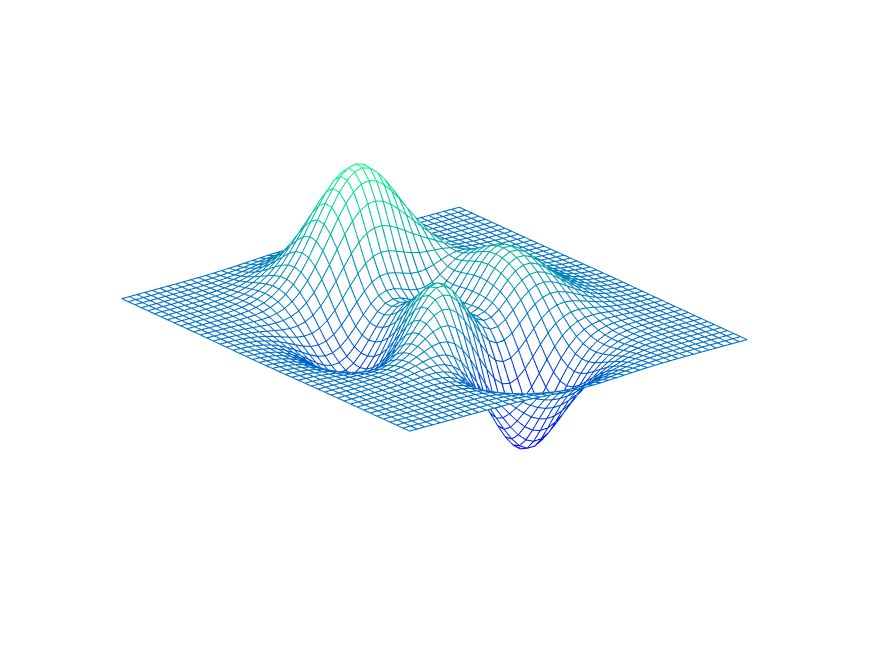
\includegraphics[trim={0cm 0cm 0cm 0cm},clip,height=0.2\textheight,width=1\linewidth,keepaspectratio]{../Figures/exfigure1} \\
							\end{center}
							\vspace{-0.5cm}
							\caption{Subfigure A} \label{subfig:exsubfigureA}
							\vspace{0.5cm}
						\end{subfigure}
						
						\begin{subfigure}[t]{\linewidth}
							\begin{center}
								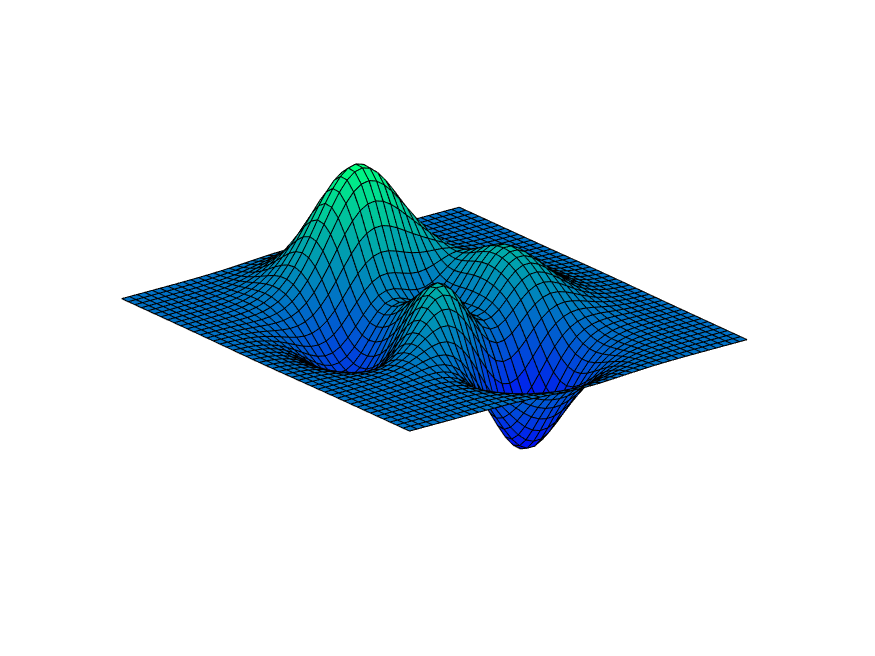
\includegraphics[trim={0cm 0cm 0cm 0cm},clip,height=0.2\textheight,width=1\linewidth,keepaspectratio]{../Figures/exfigure2} \\
							\end{center}
							\vspace{-0.5cm}
							\caption{Subfigure B} \label{subfig:exsubfigureB}
							\vspace{0.5cm}
						\end{subfigure}
					\fignotes{Add standalone description. You can reference sections like \ref{sec:data} and variables like \lastobs.} 
				\end{minipage}
			\end{center}
		\end{figure}
%	}
\end{document}
% trim = {<left> <lower> <right> <upper>}

\end{appendices}